\documentclass[journal]{IEEEtran}

% *** CITATION PACKAGES ***
%
%\usepackage{cite}
\usepackage{capt-of}%%To get the caption
\usepackage{gensymb}
\usepackage{graphicx} %package to manage images
\graphicspath{ {./images/} }
\usepackage{wrapfig}

\usepackage[style=ieee]{biblatex}
\DeclareLanguageMapping{english}{english-apa}
\addbibresource{references.bib}
\usepackage[justification=centering]{caption}

\usepackage{setspace}

\usepackage{hhline}

\usepackage{booktabs}

% *** GRAPHICS RELATED PACKAGES ***
%
\ifCLASSINFOpdf
  % \usepackage[pdftex]{graphicx}
  % declare the path(s) where your graphic files are
  % \graphicspath{{../pdf/}{../jpeg/}}
  % and their extensions so you won't have to specify these with
  % every instance of \includegraphics
  % \DeclareGraphicsExtensions{.pdf,.jpeg,.png}
\else
  % or other class option (dvipsone, dvipdf, if not using dvips). graphicx
  % will default to the driver specified in the system graphics.cfg if no
  % driver is specified.
  % \usepackage[dvips]{graphicx}
  % declare the path(s) where your graphic files are
  % \graphicspath{{../eps/}}
  % and their extensions so you won't have to specify these with
  % every instance of \includegraphics
  % \DeclareGraphicsExtensions{.eps}
\fi
% graphicx was written by David Carlisle and Sebastian Rahtz. It is
% required if you want graphics, photos, etc. graphicx.sty is already
% installed on most LaTeX systems. The latest version and documentation
% can be obtained at: 
% http://www.ctan.org/pkg/graphicx
% Another good source of documentation is "Using Imported Graphics in
% LaTeX2e" by Keith Reckdahl which can be found at:
% http://www.ctan.org/pkg/epslatex
%
% latex, and pdflatex in dvi mode, support graphics in encapsulated
% postscript (.eps) format. pdflatex in pdf mode supports graphics
% in .pdf, .jpeg, .png and .mps (metapost) formats. Users should ensure
% that all non-photo figures use a vector format (.eps, .pdf, .mps) and
% not a bitmapped formats (.jpeg, .png). The IEEE frowns on bitmapped formats
% which can result in "jaggedy"/blurry rendering of lines and letters as
% well as large increases in file sizes.
%
% You can find documentation about the pdfTeX application at:
% http://www.tug.org/applications/pdftex

\begin{document}

\begin{titlepage}
    {\centering
        \vspace*{20em}
        {
        \huge 
        \begin{spacing}{1.5}
            Lab Report \#5: LC Circuit
            \\
            Circuits Fundamentals Lab, Spring 2019
            \bigskip
            \Large
            \\
            Determining the Inductance of a Built Inductor\\
            By Analysis of a Simple Inductor-Capacitor (Tank) Circuit
  
            \\
            \bigskip
            Deadline: March 6, 2019 
        \end{spacing}

        }
        
    }
    \vfill
    
    {
    \large
    
    \begin{spacing}{1.5}
    \noindent Barkin Simsek, {\it {bs3528@nyu.edu}} 
    \\
    Nishant Aswani, {\it {nsa325@nyu.edu}}
    \\
    Section \#1% <-this % stops a space
    \\
    Workstation \#8% <-this % stops a space
    \end{spacing}
    }


\end{titlepage}
\pagenumbering{gobble}
%\clearpage\mbox{} % adds and empty page
%\clearpage
\pagenumbering{arabic}
\setcounter{page}{1}

%\title{Demonstration of a Voltage Divider With A Variable Resistor}

%\author{Barkin Simsek,~\IEEEmembership{bs3528@nyu.edu};
%Nishant Aswani,~\IEEEmembership{nsa325@nyu.edu}
%\\ Table Number: \#}% <-this % stops a space


% The paper headers
\markboth{Simsek, Aswani, Circuits Fundamentals Lab 2019}%
{}

% make the title area
%\maketitle

% As a general rule, do not put math, special symbols or citations
% in the abstract or keywords.
\begin{abstract}
In this experiment, an inductor was built by using copper wire and PVC pipe. The inductor was used to implement a simple LC circuit, through which AC signals were passed at varying frequencies and the output was measured using an oscilloscope, thus allowing for the calculation of the resonant frequency and inductance. Calculations showed that the resonant frequency for the built inductor was 14400 Hz; therefore, the calculated inductance was 0.083 mH. This was compared to the measured inductance of 0.081 mH, thus verifying the experimental procedure as a valid method for determining an unknown inductance.
\end{abstract}

%Percenta of power being consumed at the internal resistence

%What happens to voltage when external load is connected and current %consumption increaased

%Formula derivation
%Application 


\section{Introduction}

\IEEEPARstart{T}\lowercase{he} goal of this lab was to build an inductor and connect it to a simple inductor-capacitor (LC) circuit. In doing so, the aim was to determine the resonance frequency ($F_{r}$) of the circuit and thus determine the inductance of the built inductor.\\

\noindent As current passes through the coil in the inductor, a magnetic field, and thus a magnetic flux, is generated through the core. Increasing or decreasing the current, produces a change in the magnetic field, which is followed by the generation of an electric field \cite{inductors}. Thus, while an inductor acts as a short-circuited wire to direct current (DC), the main quality of the passive component is that it opposes the changing of current direction through it \cite{hayt1986engineering}, which is what alternating current (AC) provides. Following this, an inductor is incapable of having an abrupt or non-continuous change in current passing through it. Moreover, looking at equation \ref{eq:inductorTheory}, an infinite change in current would require an infinite voltage, which is physically impossible.


\begin{equation}
v = L\frac{di}{dt}
\label{eq:inductorTheory}
\end{equation}


\noindent When an inductor is connected in parallel with a capacitor and power is supplied using an AC function generator (see Figure \ref{fig:c1}), then there are two extreme scenarios, which depend on the frequency of the provided alternating current.

% \noindent In direct current (DC) circuits, capacitors are used as "storage devices" to collect charge as long as a voltage is constantly applied. On the other hand, in alternating current (AC) circuits, the capacitor charges and discharges as the current alternates. This charging and discharging behavior occurs in a 90\degree  phase difference to the alternating current. Due to different behavior based on either DC or AC, capacitors are often used in high pass (HPF) and low pass filters (LPF) to filter out certain signals. The placement of capacitors in HPF and LPF is shown in Figures \ref{fig:HPF} and \ref{fig:LPF}.


\begingroup
    \centering
    \medskip
    %width=\columnwidth
    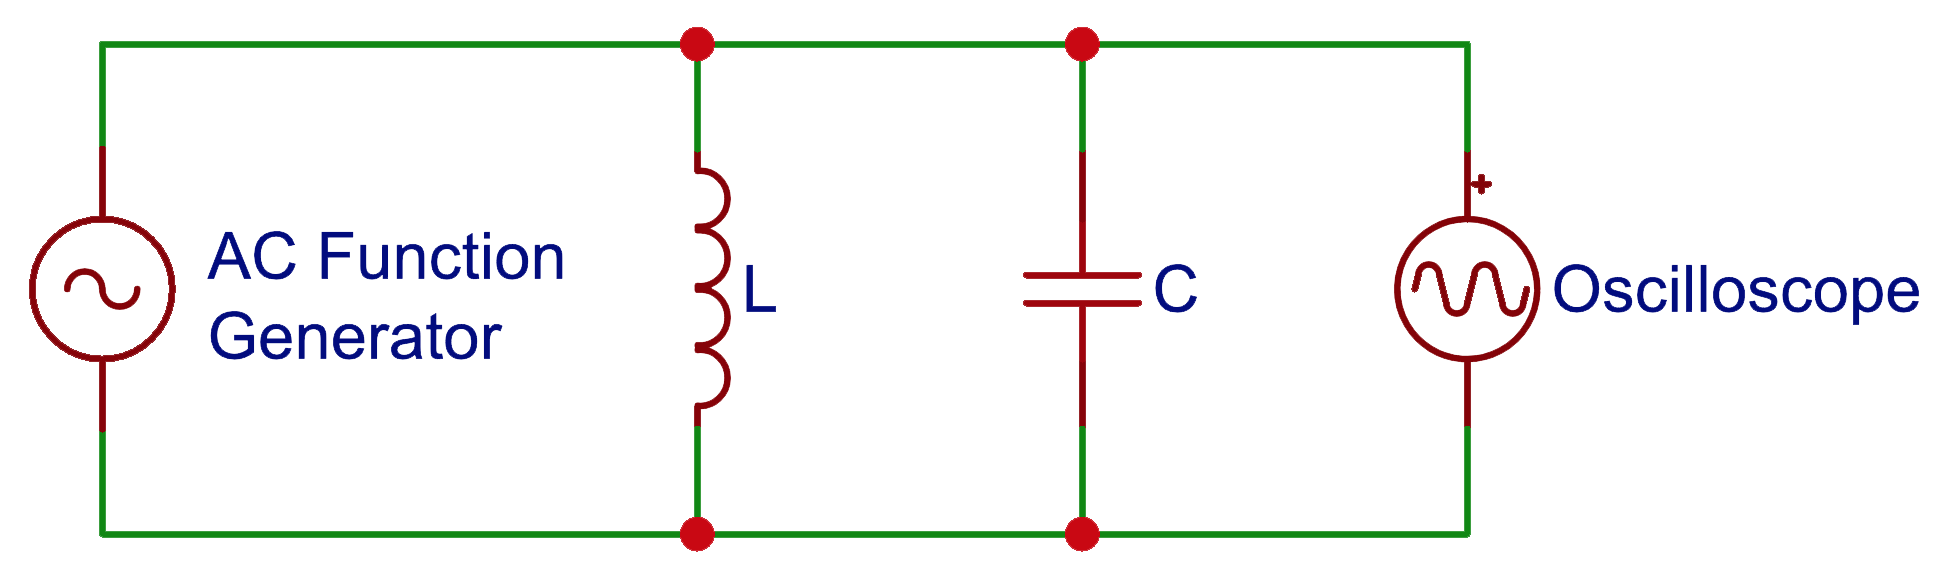
\includegraphics[width=\columnwidth]{images/lab5_6.png}
    \captionof{figure}{A simple inductor-capacitor (tank) circuit}
    \label{fig:c1}
    \medskip
\endgroup

\noindent In one extreme, where the supplied current is of very low frequency, the inductor acts as a short-circuiting wire while the capacitor acts as an open circuits (see Figure \ref{fig:c2}). 

\begingroup
    \centering
    \medskip
    %width=\columnwidth
    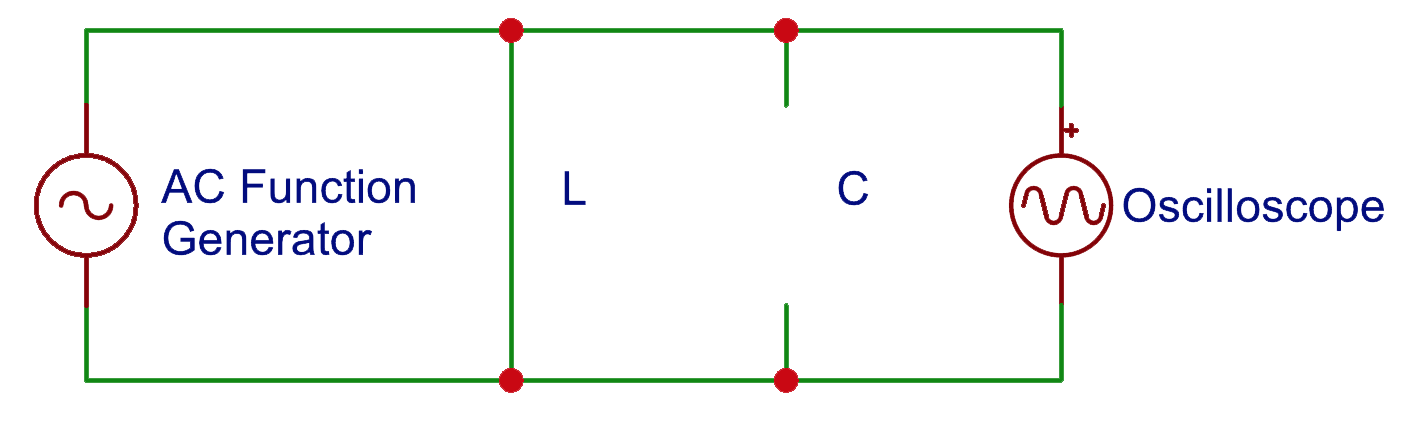
\includegraphics[width=\columnwidth]{images/lab5_8.png}
    \captionof{figure}{Extreme case of very low frequency}
    \label{fig:c2}
    \medskip
\endgroup

\noindent On the other hand, when the supplied current is of very high frequency, the inductor acts an open-circuiting element, as inductors oppose change, while the capacitor acts a short-circuiting element (see Figure \ref{fig:c3}).

\begingroup
    \centering
    \medskip
    %width=\columnwidth
    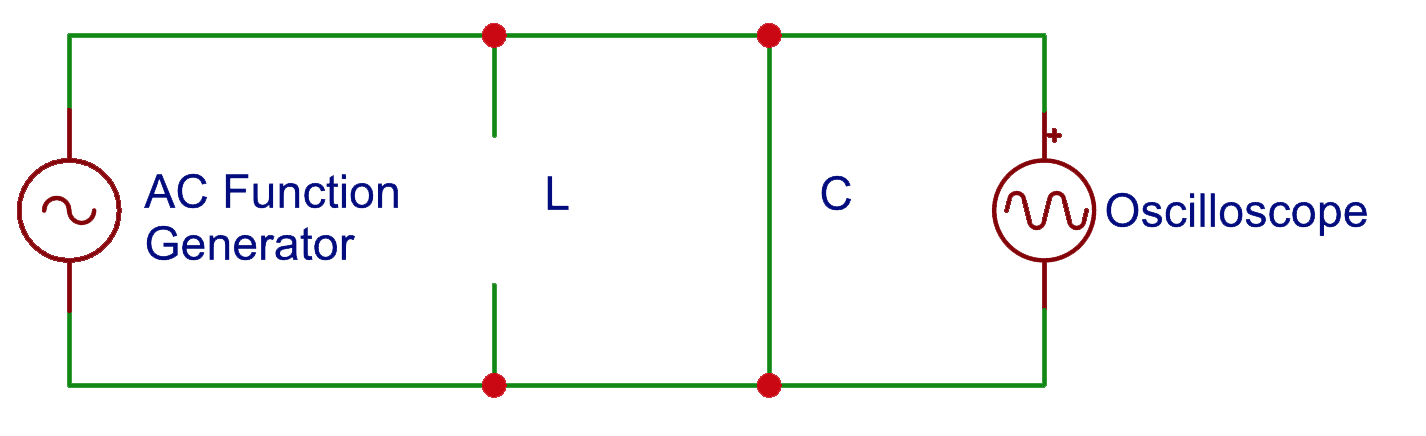
\includegraphics[width=\columnwidth]{images/lab5_9.png}
    \captionof{figure}{Extreme case of very high frequency}
    \label{fig:c3}
    \medskip
\endgroup

\noindent In each of the extreme cases, one of the two components reaches its maximum impedance. There must also then exist a certain frequency, the resonance frequency $(F_{r})$, at which the impedance of both components is at its maximum. In the case of resonance frequency, the circuit effectively is open-circuited. Therefore, theoretically, all the current circulates between the two components and the output voltage is equal to the input voltage \cite{equations}.\\

\noindent If X represents impedance:


\begin{equation}
X_{L}=2\pi fL
\label{eq:XL}
\end{equation}

\begin{equation}
X_{c}=\frac{1}{2\pi fC}
\label{eq:XC}
\end{equation}

\noindent Then, setting the two impedances equal to each other and simplifying the equation leads to an equation that determines the resonance frequency \cite{equations}.

\begin{equation}
F_{r}=\frac{1}{2\pi \sqrt{LC}}
\label{eq:FR}
\end{equation}

\noindent Experimentally determining the resonance frequency and manipulating Equation \ref{eq:FR} can then help in calculating the unknown inductance of the built inductor.

\section{Building the Inductor and Tank Circuit}

\noindent An inductor is simply a coil of conductor wrapped around a core. The built inductor used copper wires wound around PVC pipes, ensuring that the windings were as taut and parallel to each other as possible. To allow for this, four PVC joints each had ten grooves sawed into them. The PVC joints were then attached to the four ends on a cross-shaped PVC pipe. Then, the copper wire was tightly wound around the PVC piece ten times and each winding was placed into the grooves (see Figure \ref{fig:inductor}).\\

\noindent To build the filtering circuit, the schematic from Figure \ref{fig:c1} was simply followed. In short, the power cable from the AC function generator was connected to one terminal of the built inductor and a $1.5\mu F$ capacitor, finally connecting to the power input of the oscilloscope. Similarly, the negative terminal was connected to the remaining terminal of the inductor and capacitor and connected to the negative terminal of the oscilloscope, grounding everything (see Figure \ref{fig:Process}).


\begingroup
    \centering
    \medskip
    %width=\columnwidth
    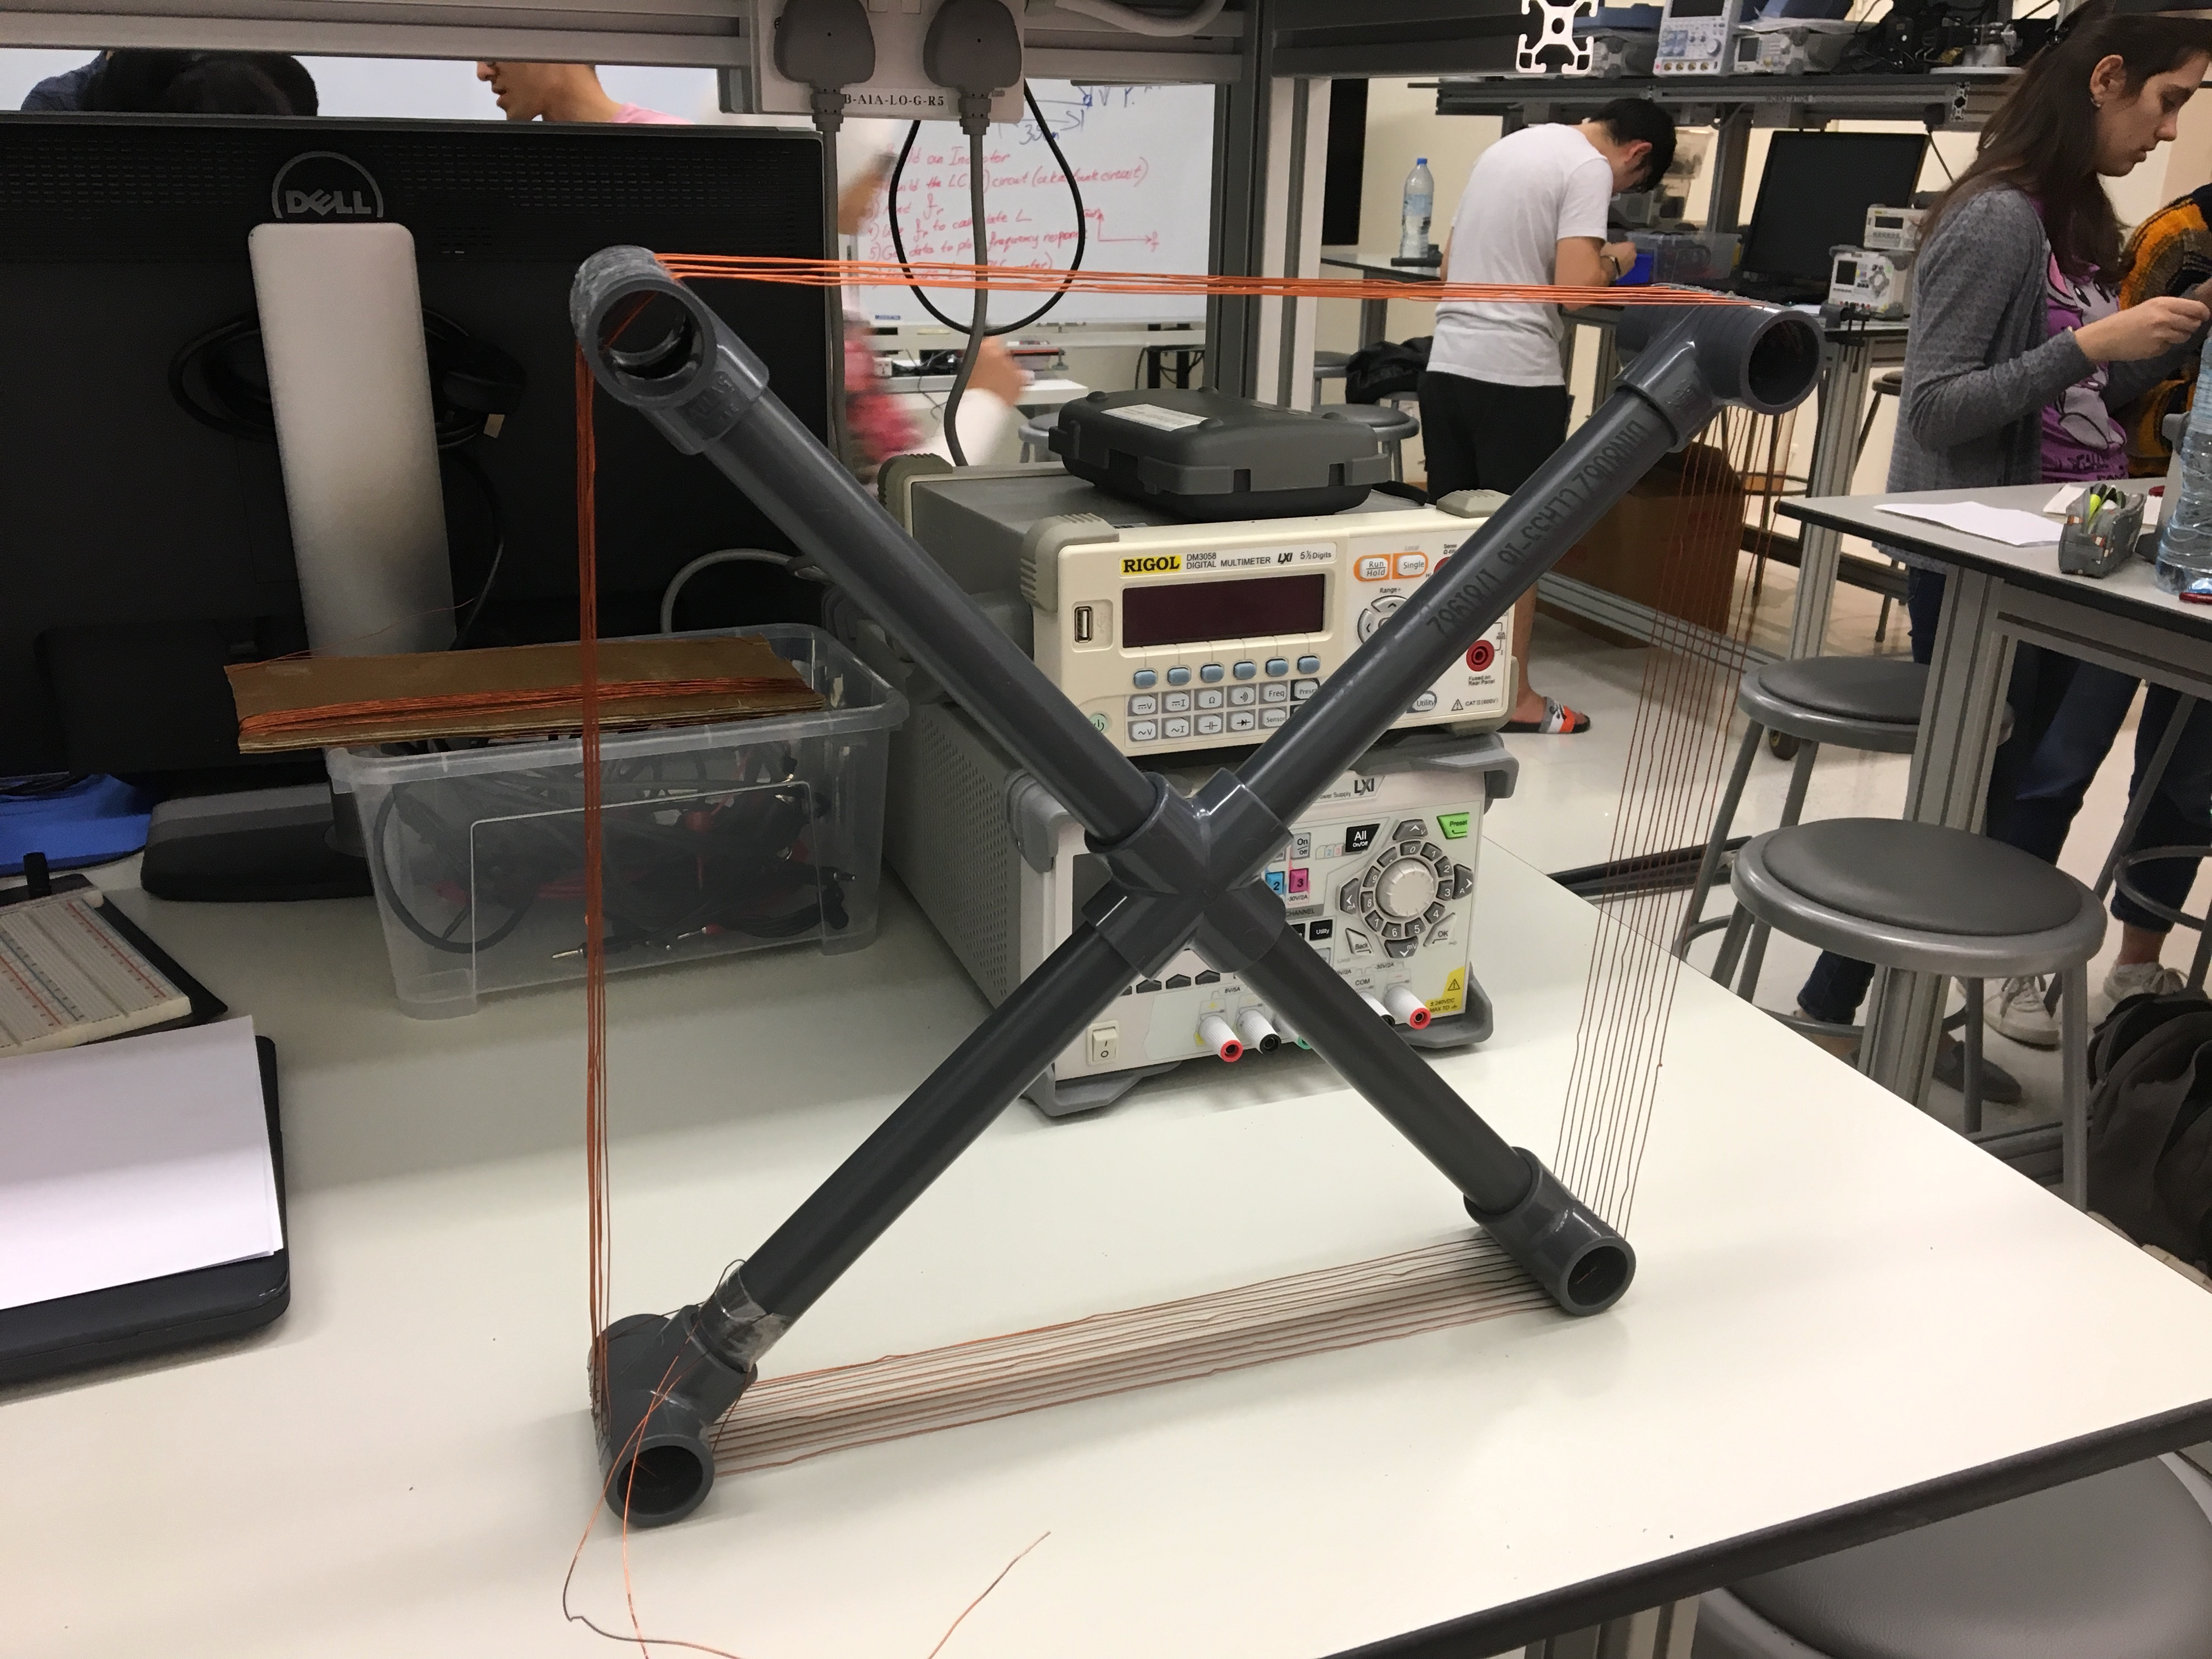
\includegraphics[width=245]{images/lab5_1.jpg}
    \captionof{figure}{Final built inductor.}
    \label{fig:inductor}
    \medskip
\endgroup

\begingroup
\medskip
    \centering
    %width=\columnwidth
    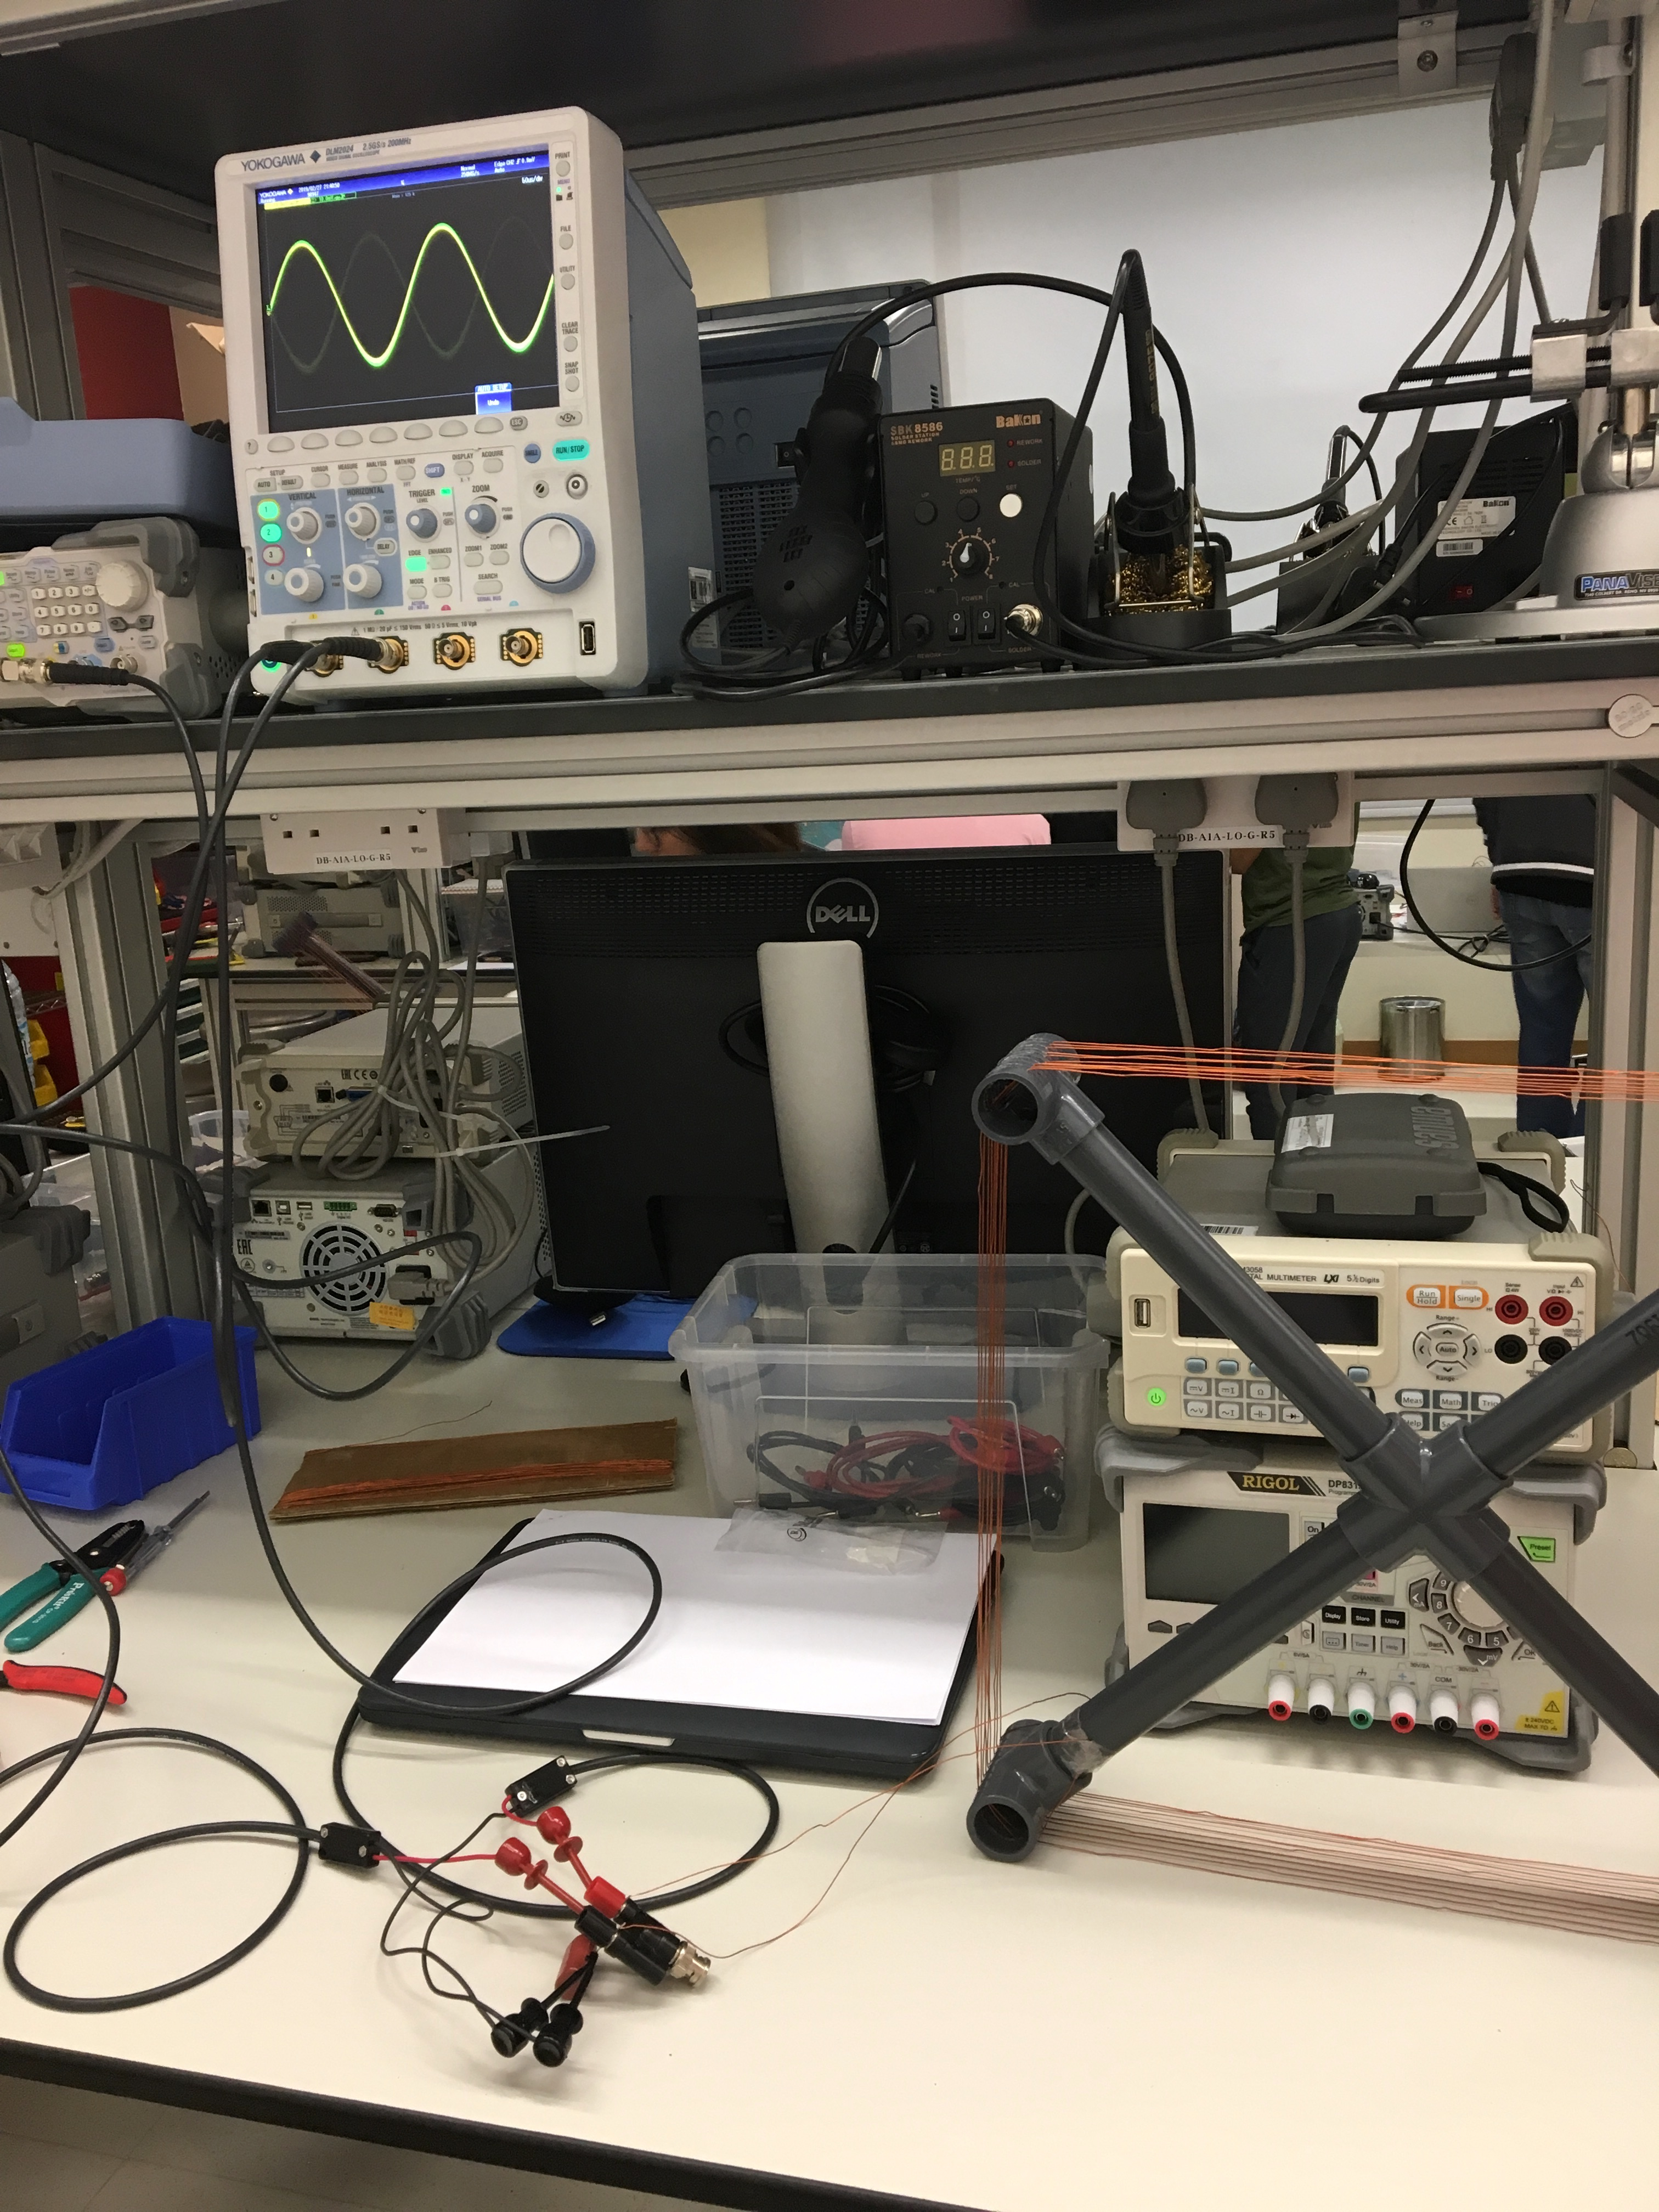
\includegraphics[width=245]{images/lab5_2.jpg}
    \captionof{figure}{Connecting the built inductor to the parallel tank circuit.}
    \label{fig:Process}
    \medskip
\endgroup

\section{Results}

\noindent To carry out the experiment and determine the $F_{r}$, the output voltage from the AC functiong generator was set to a constant $1V$. Then, beginnining at 5k Hz, the input frequency of the signal was incremented and the output voltage read by the oscilloscope was recorded, producing the data seen in Figure \ref{fig:table}. Although, theoretically, the output voltage is to be equivalent to the input voltage at resonance frequency, the data produced showed a clear increase and decrease in gain (the ratio of output voltage to input voltage. 


\begingroup
    \centering
    \medskip
    \def\arraystretch{1.5}
    \begin{tabular}{cc}
    \hline
    Frequency (Hz) & Gain \\
    \hline
    5k & 0.062 \\
    6k & 0.078 \\
    7k & 0.096 \\
    8k & 0.118 \\
    9k & 0.148 \\
    10k & 0.188 \\
    11k & 0.248 \\
    12k & 0.316 \\
    13k & 0.400 \\
    14k & 0.470 \\
    15k & 0.476 \\
    16k & 0.374 \\
    17k & 0.310 \\
    18k & 0.260 \\
    19k & 0.220 \\
    20k & 0.200 \\
    21k & 0.170 \\
    22k & 0.154 \\
    23k & 0.140 \\
    24k & 0.126 \\
    25k & 0.120 \\
    26k & 0.110 \\
    27k & 0.100 \\
    28k & 0.096 \\

    \hline
    \end{tabular}
    \captionof{figure}{Tabulation of the gain against varied frequency of the input voltage (Hz) for a parallel tank circuit}
    \label{fig:table}
    \medskip
\endgroup

\noindent Figure \ref{fig:graph} graphs the data found in the table, elucidating the relationship between frequency and gain (or impedance). Clearly, at lower frequencies the inductor has a greater effect of drawing on the current, as most of the impedance comes from the capacitor. At higher frequencies, the capacitor draws on the current and only the inductor provides impedance. 

\noindent As highlighted in Figure \ref{fig:graph}, the resonance frequency was determined to be at approximately \textbf{14,400 Hz}.

\noindent Using the gathered data, Equation \ref{eq:FR} was manipulated to produce the following equation:

\begin{equation}
L=(\frac{1}{2\pi F_{r}})^2 \cdot \frac{1}{C}
\label{eq:manipulateFR}
\end{equation}

\begingroup
    \centering
    \medskip
    %width=\columnwidth
    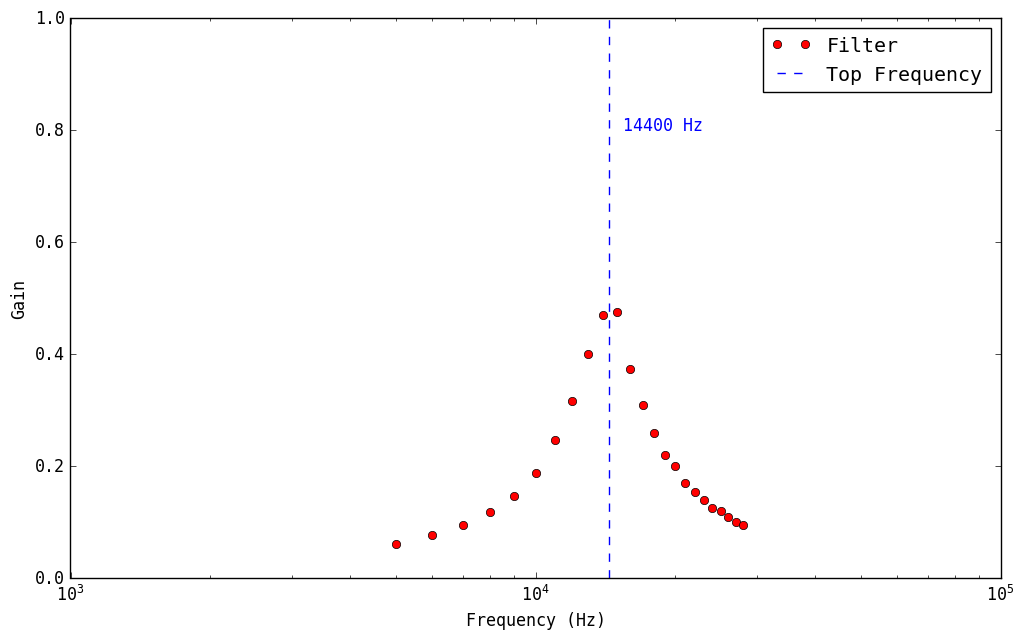
\includegraphics[width=245]{images/lab5_7.png}
    \captionof{figure}{Visual representation of the gain against frequency (Hz). The blue line depicts the resonance frequency, where the gain was at maximum}
    \label{fig:graph}
\endgroup

\noindent Replacing with known data, where $F_{r}$ is replaced with 14,400 Hz and C is replaced with 1.5 \mu F : 

\begin{equation}
L=(\frac{1}{2\pi \cdot 14400})^2 \dot \frac{1}{1.5 \cdot 10^{-6}} = 0.081 mH
\label{eq:manipulateFR}
\end{equation}

\noindent The calculation led to an experimentally determined value of 0.081 milliHenries (mH). The inductance of the inductor was also measured with an LCR meter and was found to be 0.083 mH; hence, the experimental derivation of the unknown inductance was valid and a good approximation of the actual value

\noindent Figure \ref{fig:25khz} (25 kHz), \ref{fig:14khz} (14 kHz), \ref{fig:5khz} (5 kHz) all depict the varying amplitudes as a result of varying frequencies. Figure \ref{fig:14khz} (14 kHz) is the closest representation of the gain at resonance frequency, and it is clear that the output voltage, and thus the gain, is at its highest. On the other hand, Figure \ref{fig:25khz} and Figure \ref{fig:5khz} show the amplitudes at either ends of the resonance frequency peak seen in Figure \ref{fig:graph} and thus have a lower amplitude.

\begingroup
    \centering
    \medskip
    %width=\columnwidth
    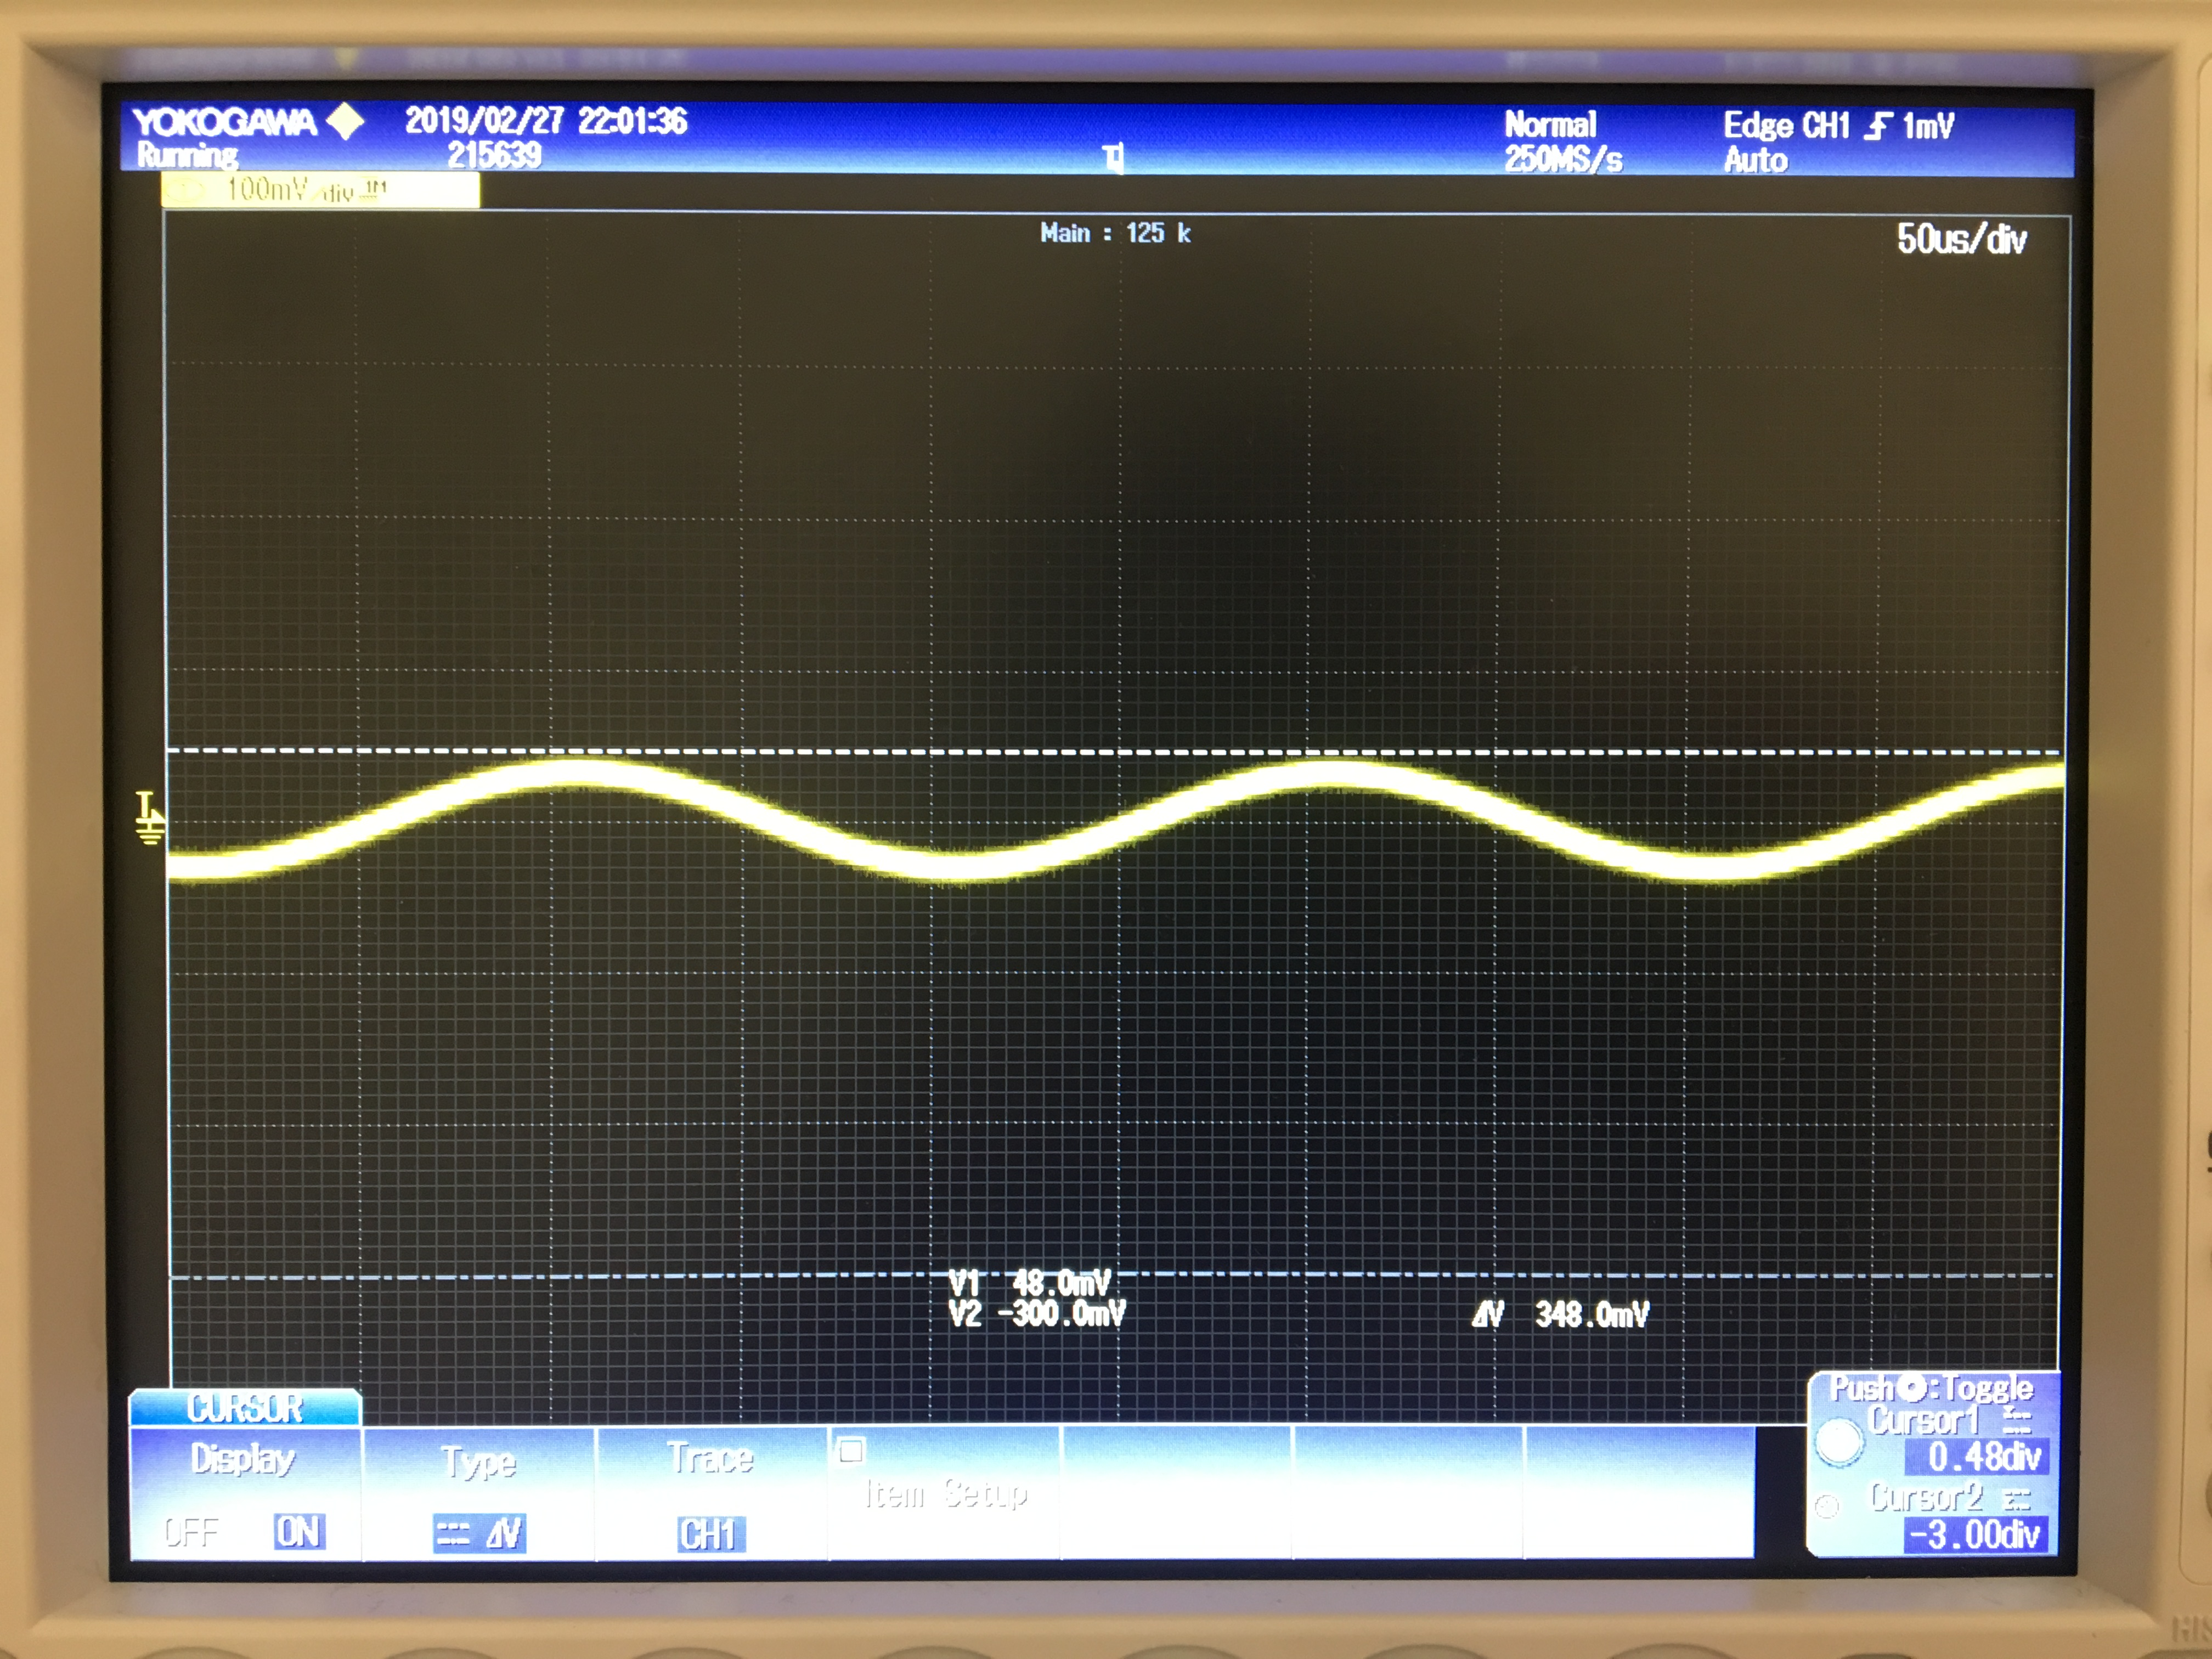
\includegraphics[width=220]{images/lab5_5.jpg}
    \captionof{figure}{The output voltage at 25 kHz input of the AC function generator}
    \label{fig:25khz}
    \medskip
\endgroup

\begingroup
    \centering
    %width=\columnwidth
    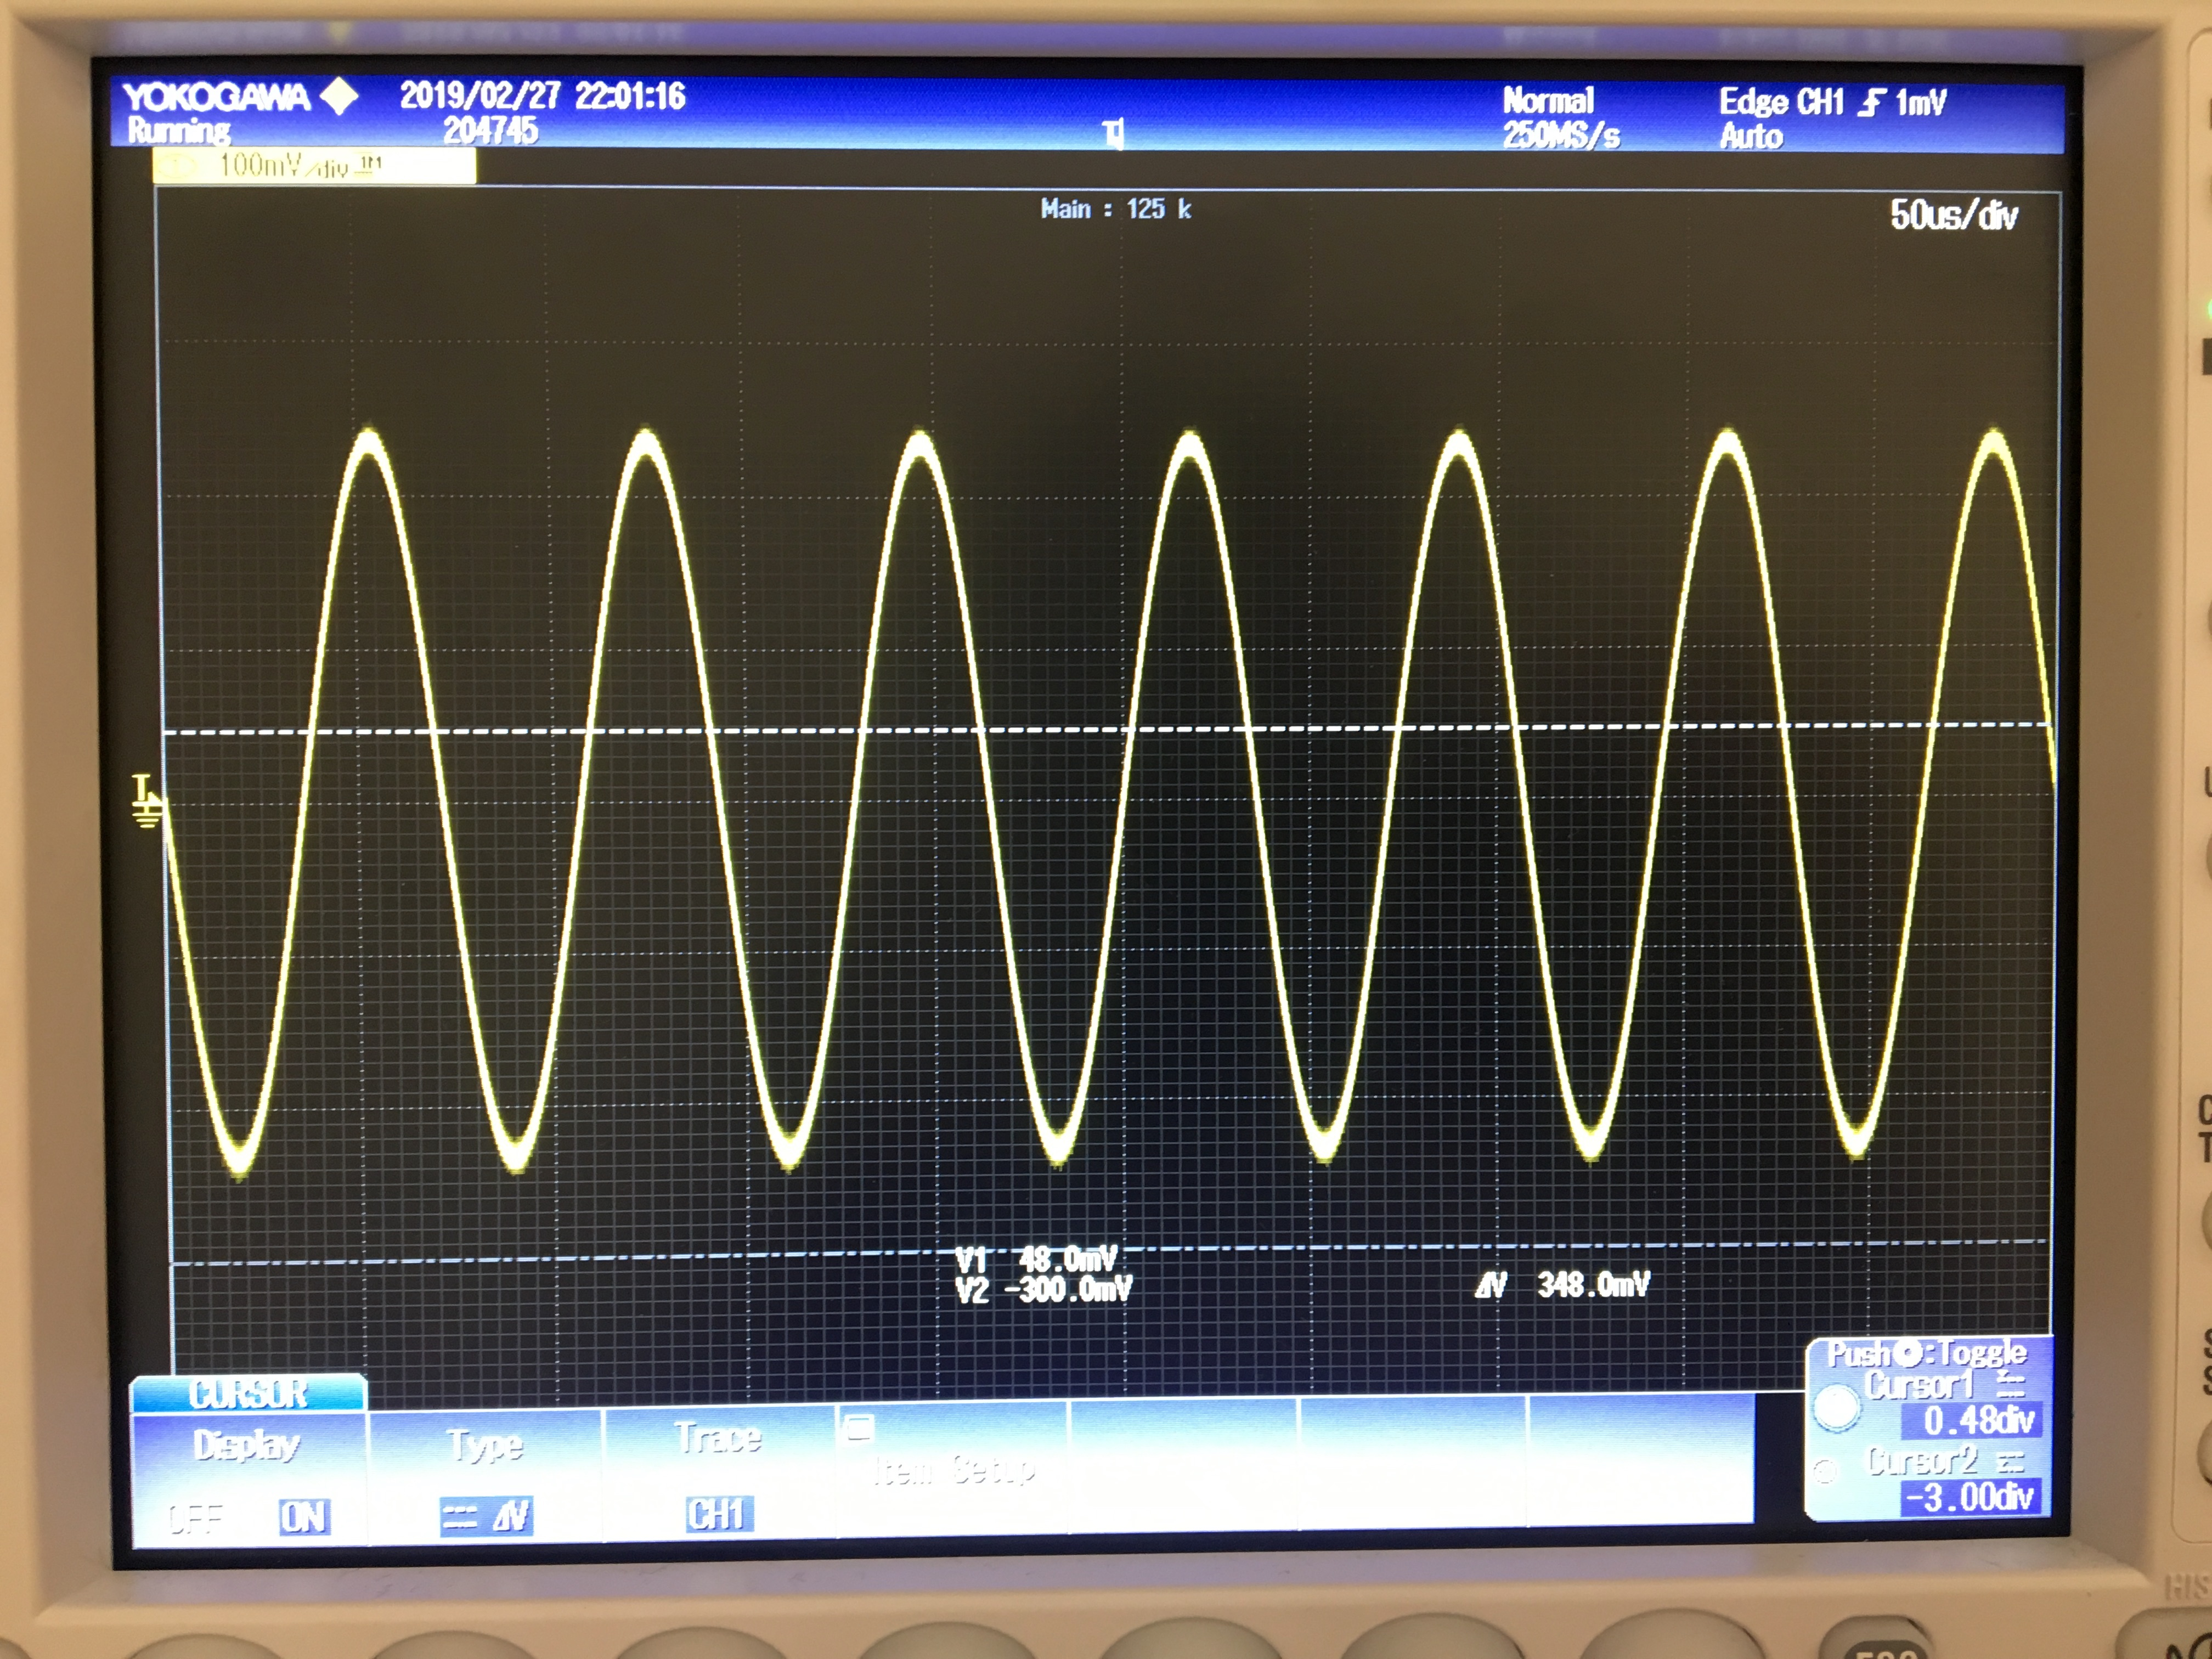
\includegraphics[width=220]{images/lab5_4.jpg}
    \captionof{figure}{The output voltage at 14 kHz input of the AC function generator}
    \label{fig:14khz}
\endgroup


\begingroup
    \centering
    %width=\columnwidth
    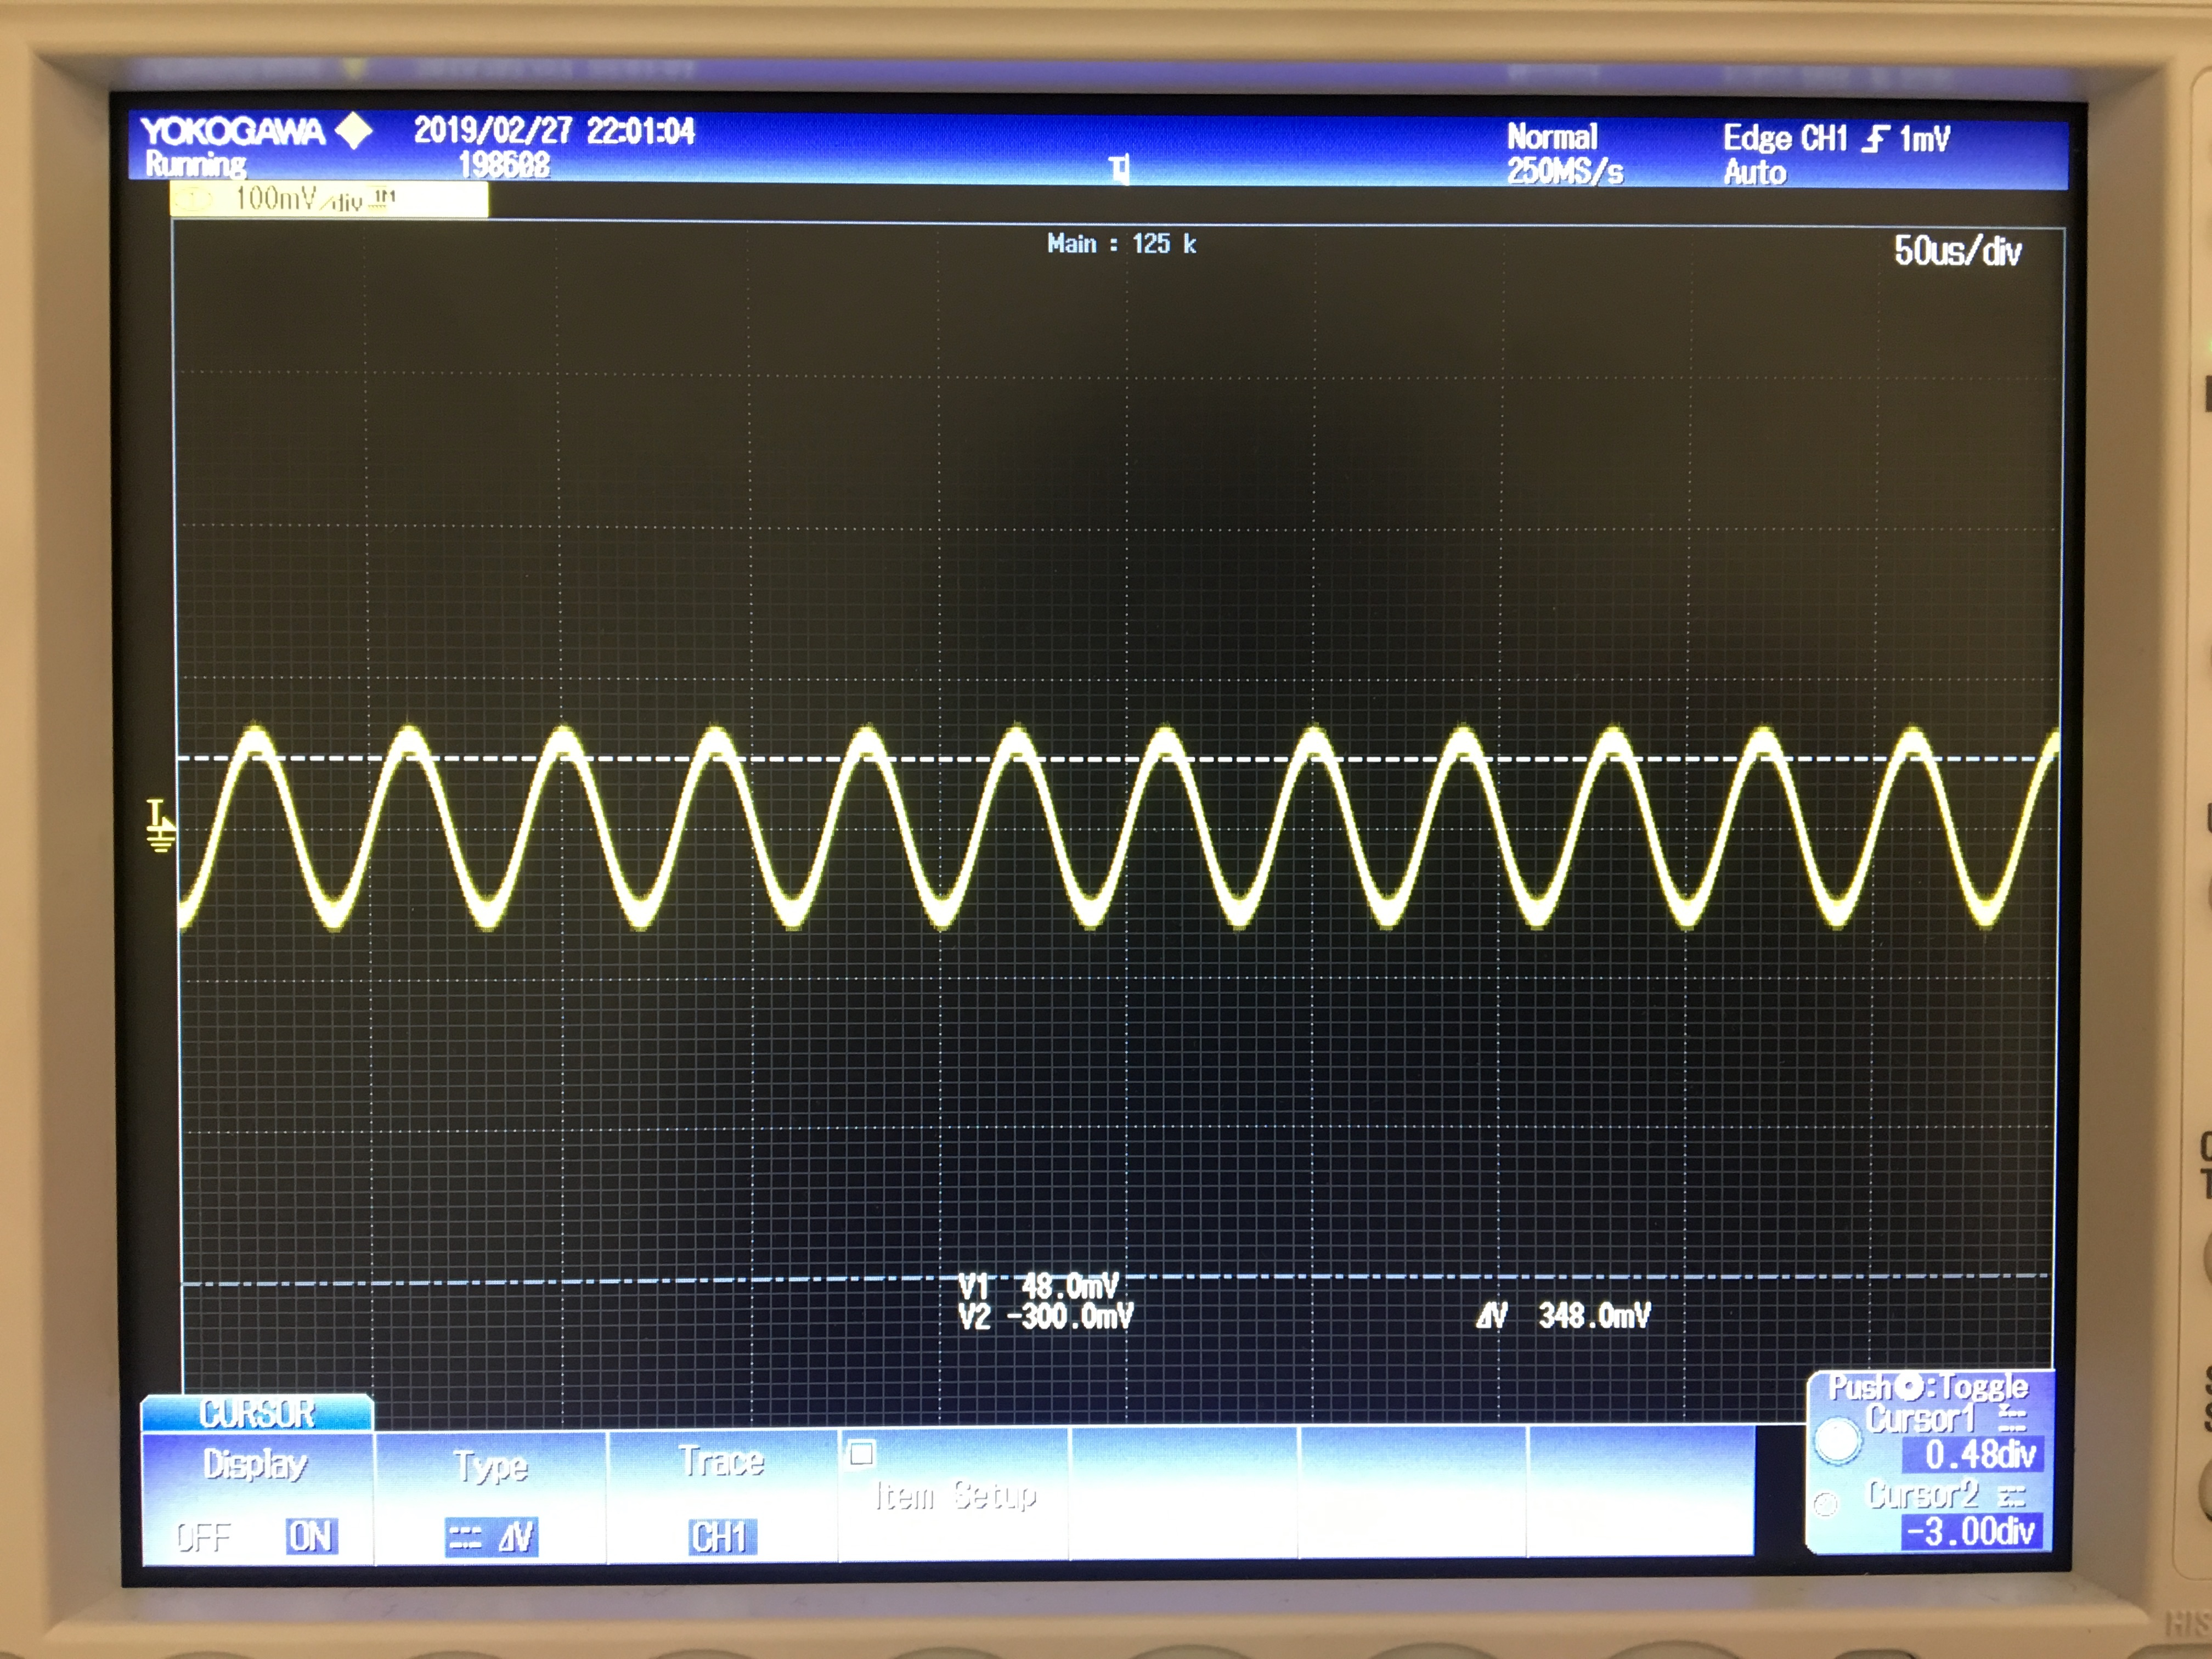
\includegraphics[width=220]{images/lab5_3.jpg}
    \captionof{figure}{The output voltage at 5 kHz input of the AC function generator}
    \label{fig:5khz}
\endgroup


\section{Conclusion} 

\noindent An inductor was built by using copper wire and PVC pipe. The built inductor was connected in parallel with a capacitor to form a simple LC circuit, also known as parallel tank circuit. A $1V$ input signal was applied across the circuit. Varying the frequency of the input signal and measuring the output voltage allowed for the measurement of gain. Gain of the built LC circuit changes based on the impedance of the $1.5uF$ capacitor and inductor built. When gain data was plotted, the resonant frequency was determined to be 14400 Hz by measuring the frequency value that gives the highest gain. Further calculations based on the measured resonant frequency showed that the inductance of the inductor is $0.081mH$. On the other hand, measuring the inductance of the inductor with an LCR meter gave an inductance value of $0.083mH$. The results gathered are practically same values and there is only 2\% difference between the theoretical result and the experimental result.\\

\noindent LC circuits can be used tuning for certain frequencies as they majorly block the whole spectrum except the resonant frequency. Therefore, they can be used in AM/FM radios to tune to a specific frequency and only listen signals coming at the particular frequency which would be matching the resonant frequency. By that way, more clear audio can be obtained by amplifying only the resonant frequency. They can be used in any other communication devices phone and satellites to only detect certain signals. Additionally, LC circuits can be used to generate certain frequencies. Therefore, they can also be used as radio wave transmitters.

%%%%%%%%%%%%%%%%%%%%%%%%%%%%%%%%%%%%%%%%%%%%%%

%please include information about the applications of 
%a "tank circuit in parallel" or "parallel tank circuit"

%%%%%%%%%%%%%%%%%%%%%%%%%%%%%%%%%%%%%%%%%%%55


%\appendices
%\section{Proof of the First Zonklar Equation}
%Appendix one text goes here.

%\section*{Acknowledgment}

\printbibliography

\end{document}